\subsection{Numerical stability}
As a final remark, the numerical stability of the solver is reported in figure \ref{fig:stability}. The map is produced for a spherical calculation of $^{16}$O, with varying box and mesh sizes. 
\\It's possible to observe that for a box whose side is at least $\approx 2.5$ times the nuclear radius, the solver numerical stability is loosely dependent on the box extension, but rather on the step size. This is not surprising, as the points separation in space $h$ dictates the precision of the discretized derivatives, as mentioned in section \ref{sec:finite_diff}.
\begin{figure}[h]
    \centering
    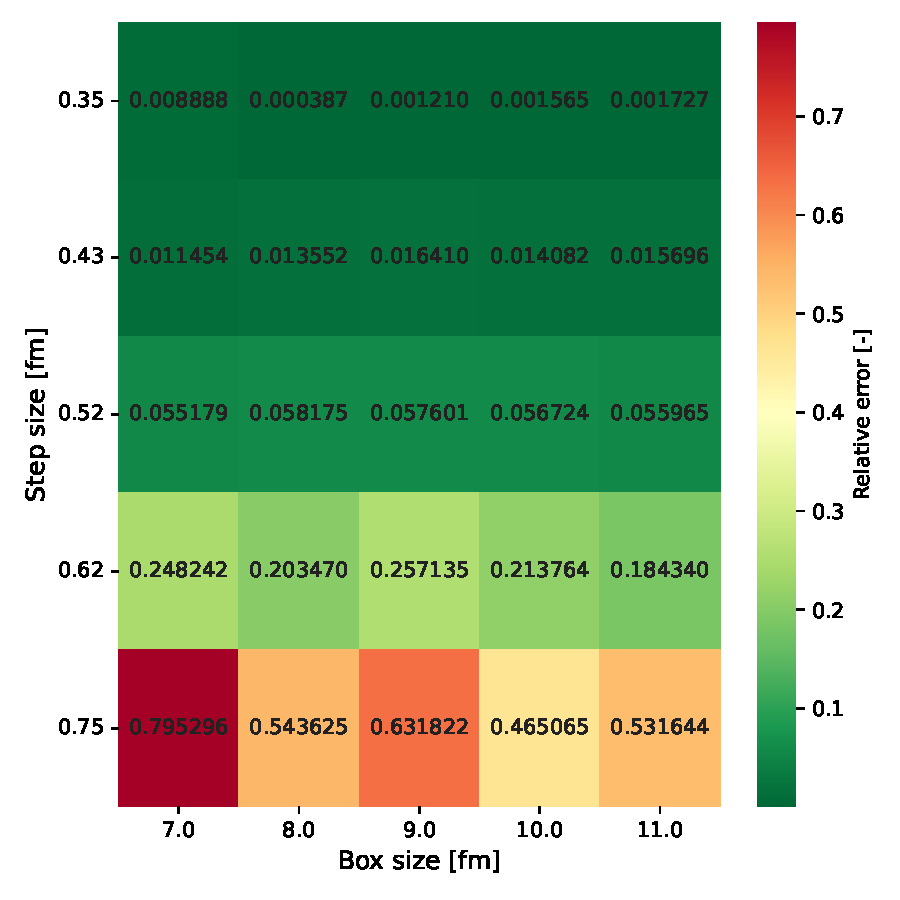
\includegraphics[width=1.0\textwidth]{Images/stability.pdf}
    \caption{Numerical stability map of the HF solver for $^{16}$O for different box and step sizes. Relative error is taken against a benchmark reference value.}
    \label{fig:stability}
\end{figure}